\section{Security Contracts approach}
\label{sec:security-contracts-approach}

\subsection{Security Contract}

\begin{equation}
SecurityContract = SecurityPattern + DbC
\end{equation}

On essaie de décrire l'approche SecurityContract indépendamment de tout langage de programmation (on pourrait le faire en n'importe quoi). Présenter donc les concepts et les aspects méthodologiques liés à ce qu'est un SecurityContract.

On y trouve pêle-mêle: des aspects structurels (avec des rôles), des aspects comportementaux, et des propriétés à garantir.

On continue en disant qu'on a choisi de faire nos expérimentations en Java, et qu'on a choisi Pamela. 

\subsection{The PAMELA framework}

Monitoring@runtime
AOP: Aspect Oriented Programming

Cf figure \ref{fig:PamelaVision}

Tout est décrit dans \cite{guerin:hal-03217126} et \cite{silva:hal-02958111}.

\begin{figure}
    \centering
    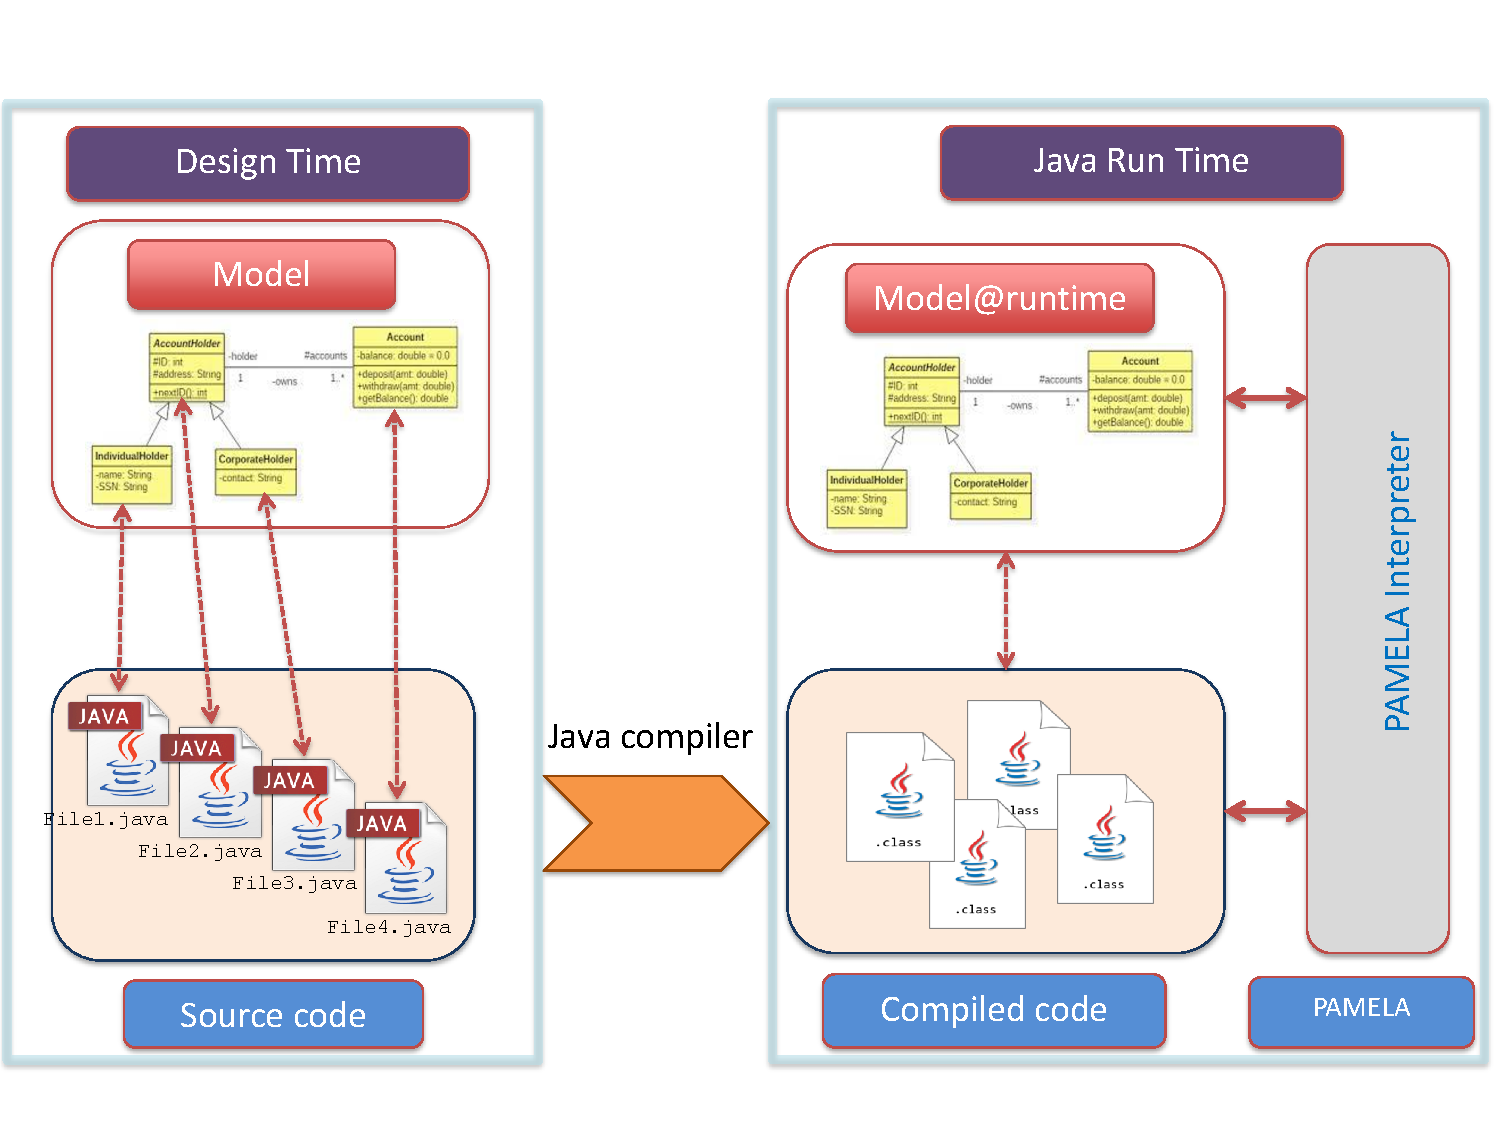
\includegraphics[width=1.0 \columnwidth]{figures/PamelaVisionV2.pdf}
    \caption{Overview of the PAMELA approach}
    \label{fig:PamelaVision}
\end{figure}

\sg{On peut peut-être glisser un petit paragraphe sur JML et l'implantation qu'on a faite dans PAMELA, en expliquant que ca marche bien, mais que c'est bien trop limité (expliquer pourquoi).}

\subsection{The \textit{Authenticator} security contract}
\label{subsec:AuthenticatorSecurityContract}

On explique l'implantation des SecurityContracts dans PAMELA.

\sg{Peut-être que le SC Authenticator peut être remonté plus haut et servir de fil rouge, ou peut-être est-ce bien de montrer qu'on parle d'une bibliothèques de SC, et que c'est juste un exemple ?}

\begin{figure}
    \centering
    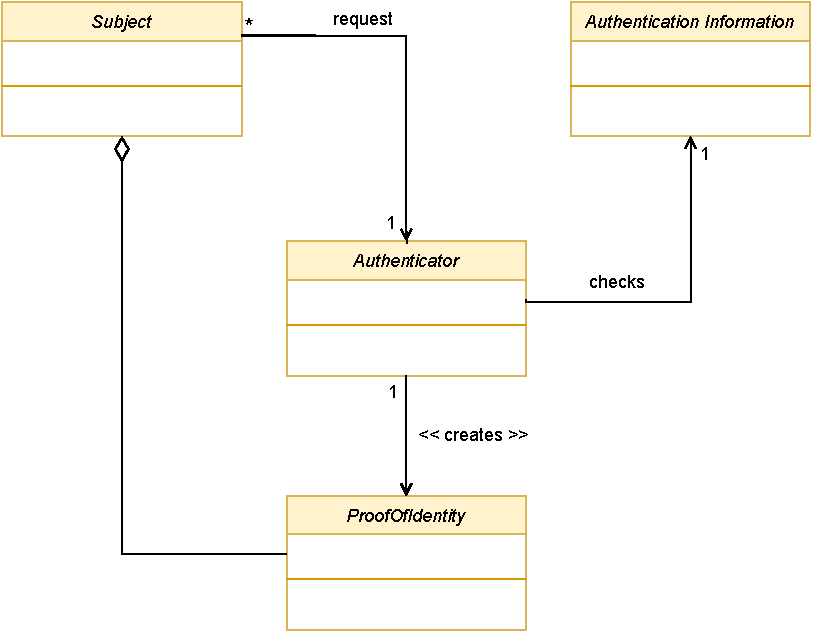
\includegraphics[width=1.0\columnwidth]{figures/AuthenticationClassDiagram.pdf}
    \caption{UML class diagram of the Authenticator security contract}
    \label{fig:authenticator_class_diagram}
 \end{figure}

\begin{figure}
    \centering
    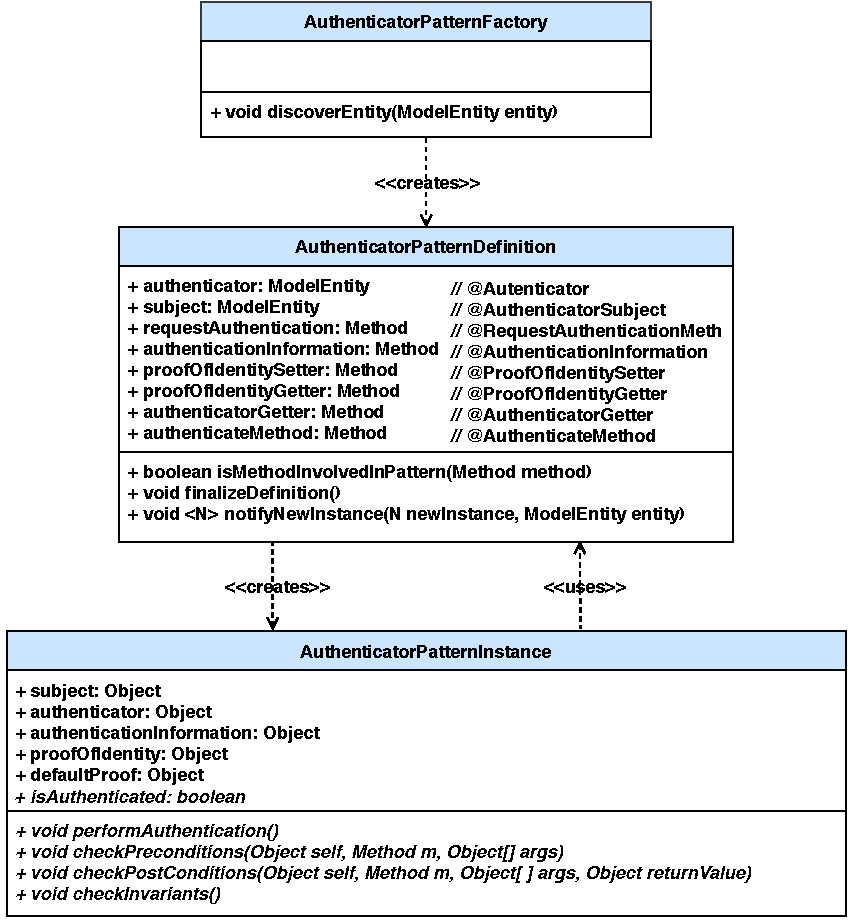
\includegraphics[width=0.8 \columnwidth]{figures/PAMELAAuthenticator_CD.pdf}
    \caption{PAMELA Authenticator pattern class diagram. Emphasized attributes and methods are the one referenced in Figure \ref{fig:AuthenticatorControlFlow}.}
    \label{fig:PAMELAAuthenticator_CD}
\end{figure}

\begin{figure}
    \centering
    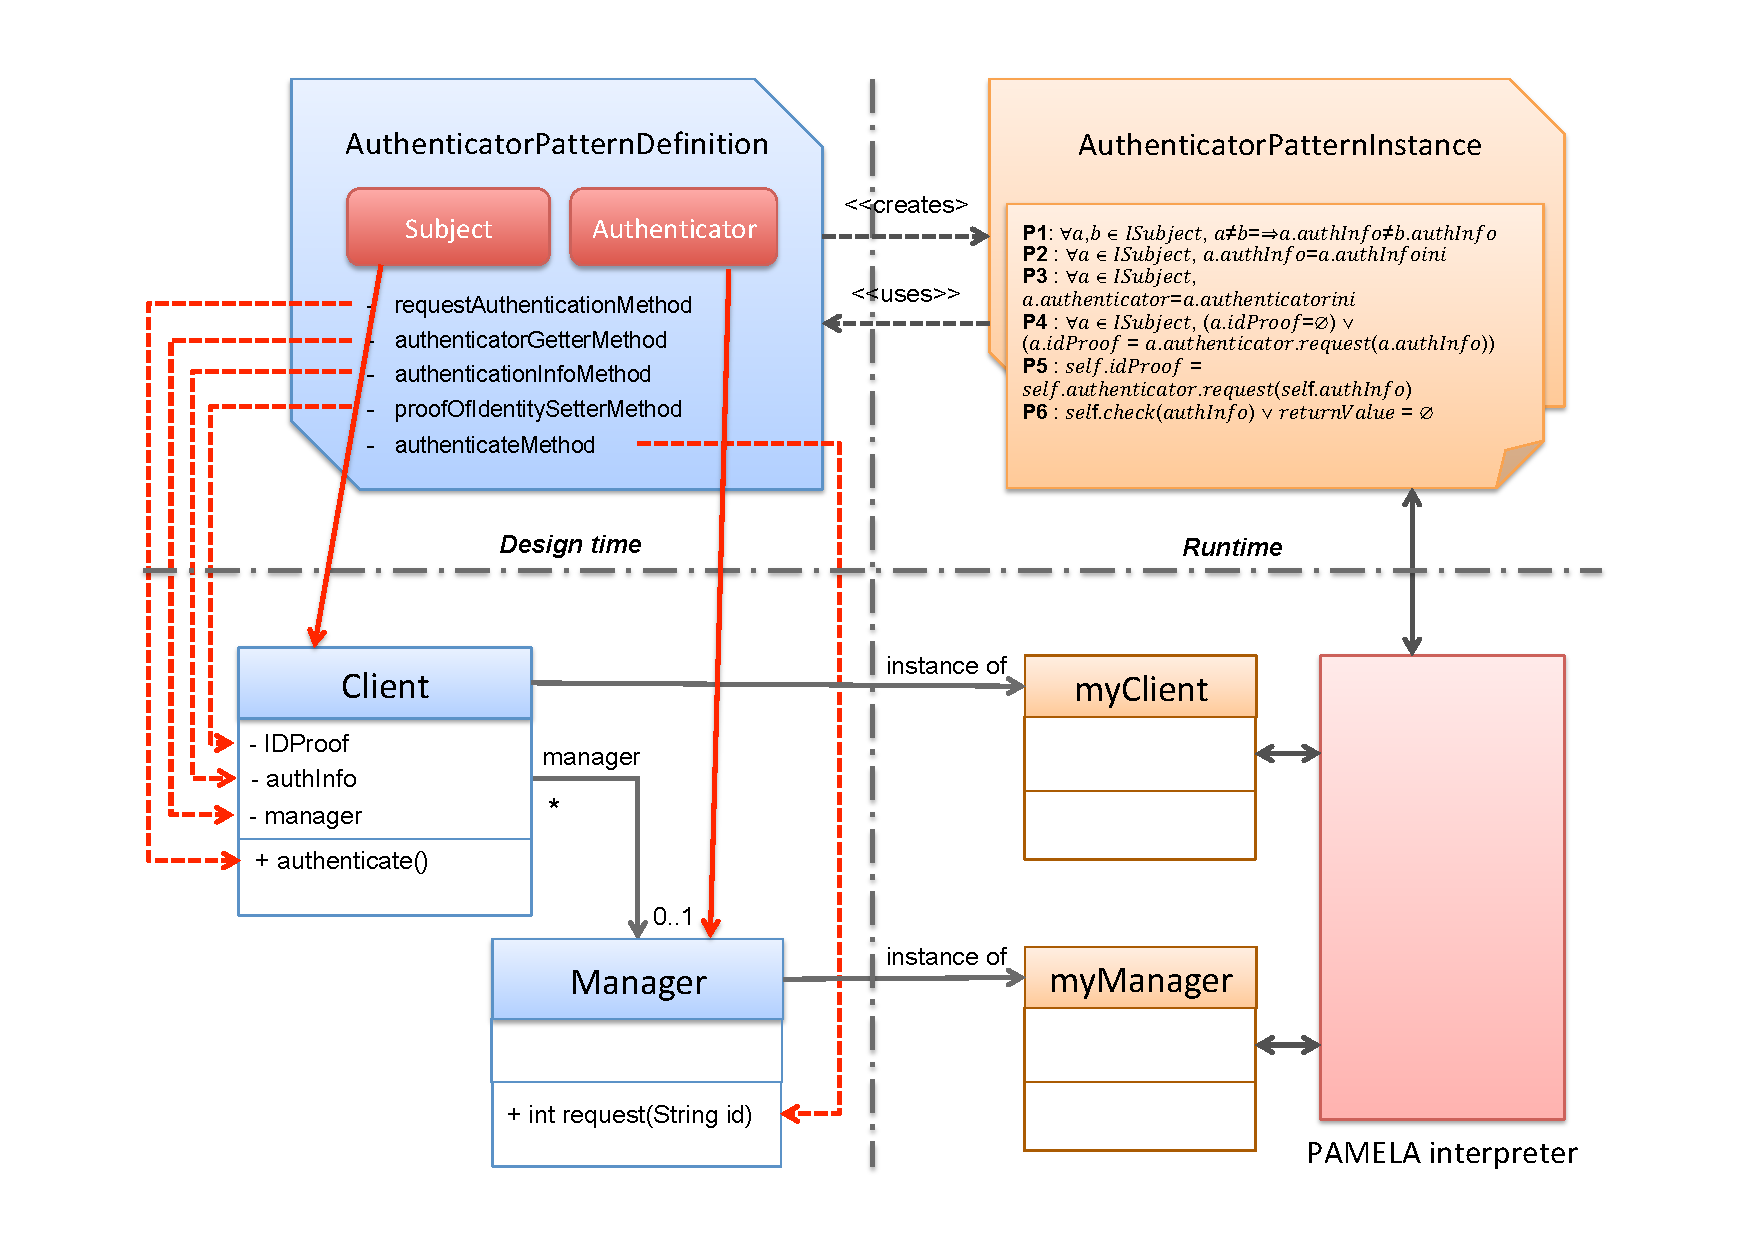
\includegraphics[width=1.0 \columnwidth]{figures/AuthenticatorPattern4.pdf}
    \caption{PAMELA vision of the authenticator pattern}
    \label{fig:AuthenticatorPattern}
\end{figure}

The excerpt of code presented Figure \ref{fig:ExampleOfAuthenticatorPattern} shows how the Authenticator pattern is used by means of annotations to an existing base of code. An instance of the \texttt{Manager} class plays the \emph{Authenticator} role, while an instance of the \texttt{Client} class plays the \emph{Subject} role.

\begin{figure}
    \centering
\begin{lstlisting}[language=Java,basicstyle=\ttfamily\footnotesize]
@ModelEntity 
@Authenticator(patternID = "PatternId")
public class Manager {

	@RequestAuthentication(patternID = "PatternId")
	public int request(@AuthenticationInformation(
        patternID = "PatternId", paramID = "id") String id) {
		return ...;
	}
}

@ModelEntity
@AuthenticatorSubject(patternID = "PatternId")
public class Client {

	public Client(Manager authenticator, String id) {
		...
	}

	@AuthenticationInformation(patternID = "PatternId", paramID = "id")
	public String getAuthInfo() {
		return ...;
	}

	@ProofOfIdentityGetter(patternID = "PatternId")
	public int getIDProof() {
		return ...;
	}

	@AuthenticatorGetter(patternID = "PatternId")
	public Manager getManager() {
		return ...;
	}

	@AuthenticateMethod(patternID = "PatternId")
	public void authenticate() {
		setIDProof(getManager().request(getAuthInfo()));
	}

	@RequiresAuthentication
	public void securedMethod() {
		...
	}
}
\end{lstlisting}
    \caption{Example showing how to use the \textit{Authenticator} defined as a PAMELA security contract}
    \label{fig:ExampleOfAuthenticatorPattern}
\end{figure}

\begin{figure}
    \centering
    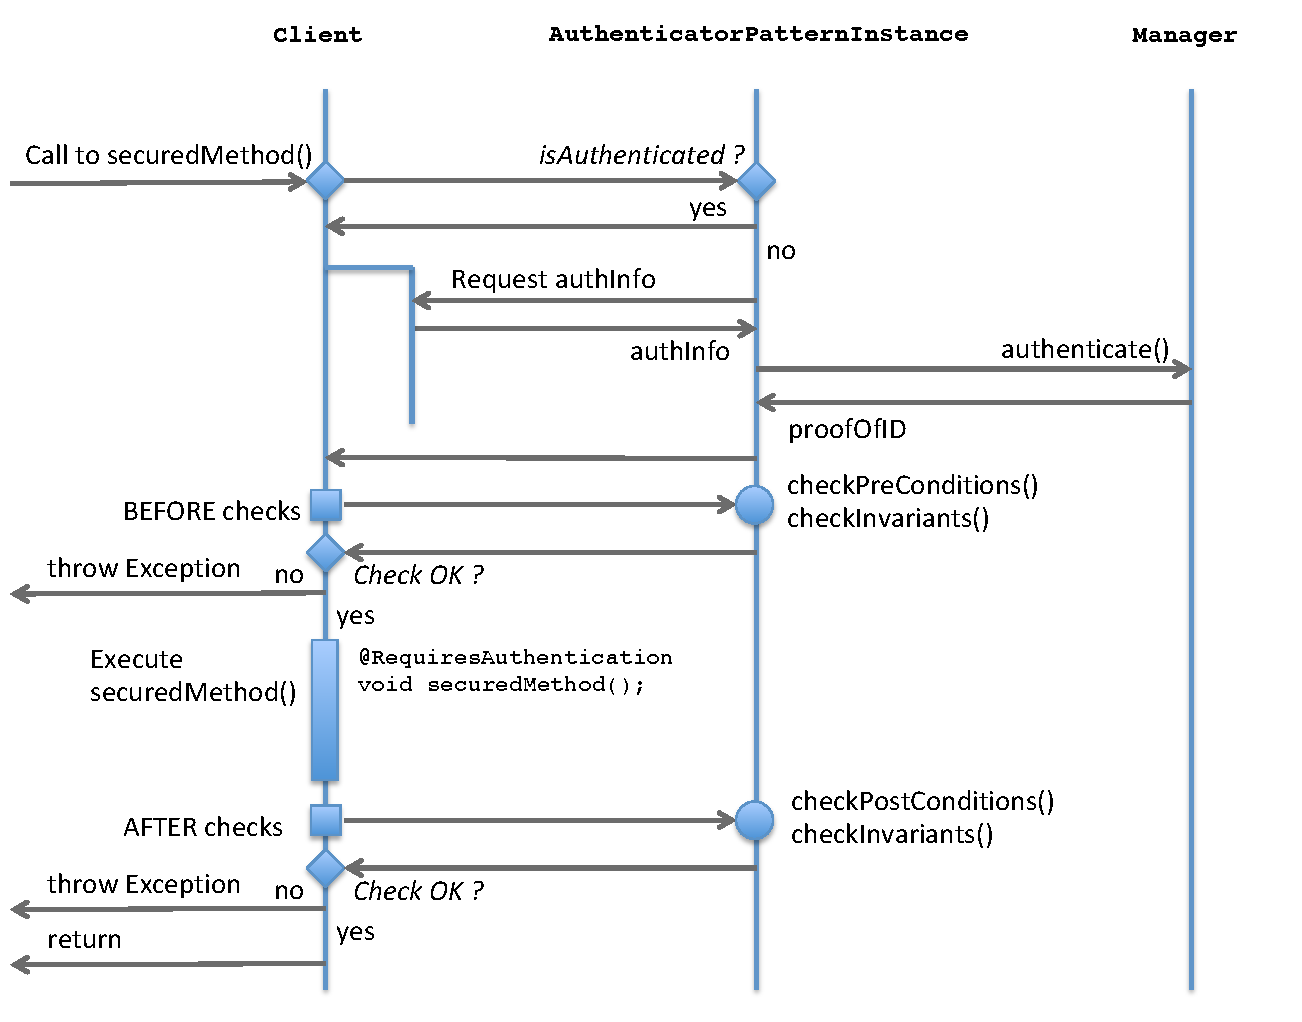
\includegraphics[width=1.0 \columnwidth]{figures/AuthenticatorControlFlow.pdf}
    \caption{Authenticator control flow}
    \label{fig:AuthenticatorControlFlow}
\end{figure}


\subsection{Security Contracts Library}

Présenter très succinctement les autres security patterns qu’on a 
Conclure en disant qu’on va se concentrer sur le seul pattern Authenticator sur un UC bien précis

A mettre peut-être dans discussion alors ?

